\documentclass[11pt]{article}
\usepackage{amsmath, amssymb, amsthm}
\usepackage{hyperref}
\usepackage{bm}
\usepackage[utf8]{inputenc}
\usepackage[T1]{fontenc}
\usepackage{times}
\usepackage{microtype}
\usepackage{graphicx}
\usepackage{amsmath,amssymb}
\usepackage{authblk}
\usepackage{geometry}
\usepackage{hyperref}
\usepackage{natbib}
\usepackage{tikz}
\usepackage{caption}
\usepackage{float}

\geometry{margin=1in}

\title{Genetic Editing as a Structural Driver of Catastrophic Collapse:\\
A Theoretical Analysis Based on Mutation Probability Structures}

\author[1]{Masaomi Chiba}
\affil[1]{Independent Researcher}
\date{}

\begin{document}
\maketitle

\begin{abstract}
This paper analyzes why modern gene editing techniques, particularly CRISPR-based systems, may pose structural risks to the long-term stability of biological lineages and ecosystems. Building on concepts from evolutionary biology and complex systems theory, we introduce the idea of a Mutation Probability Structure (MPS): the historically shaped probability distribution of permissible mutations in a lineage. Natural evolution operates within the constraints set by MPS, whereas artificial gene editing bypasses these constraints entirely. We argue that this structural bypass generates a class of risks that are difficult or impossible to observe directly, including slow ecosystem collapse, trans-generational breakdowns, and anthropic filtration (world-lines in which no observer survives). We conclude that gene editing technologies require a new ethical framework grounded not in immediate phenotypic safety, but in the preservation of long-developed evolutionary constraints.
\end{abstract}

\section{Introduction}

Gene editing technologies have achieved remarkable progress in recent years. CRISPR-Cas systems allow targeted modification of genomic sequences with unprecedented precision. These technologies promise treatments for genetic diseases, enhanced crops, and applications in synthetic biology.

However, current discussions of gene editing risks tend to focus on local issues: off-target effects, phenotypic unpredictability, ecological spread, and socioeconomic concerns. Much less attention has been given to what we call \textit{structural risks}: risks inherent not in specific edits, but in the act of bypassing the evolutionary constraints that shaped living systems over billions of years.

This paper develops a theoretical foundation for understanding these structural risks and proposes an ethics based on Mutation Probability Structure (MPS).

\section{Mutation Probability Structure (MPS)}

\subsection{Definition}

We define the \textit{Mutation Probability Structure} (MPS) as the empirically shaped probability distribution over mutations that has been reinforced through evolutionary history.

In other words:
\begin{itemize}
    \item Mutations that occur frequently tend to be compatible with lineage survival.
    \item Mutations that occur extremely rarely tend to be incompatible with lineage survival.
\end{itemize}

Thus MPS is not an "intention" of life but a structural record of what has survived natural selection.

\subsection{MPS as Evolutionary Constraint}

Because evolution is both stochastic and selective, MPS encodes:
biochemical feasibility, developmental robustness, ecological compatibility, and long-term lineage viability. Over long time scales, MPS functions as a form of deep regulatory grammar of life.

\section{Gene Editing as an MPS Bypass}

\subsection{Artificial Changes Break Probabilistic Constraints}

Natural mutation walks along the structure defined by MPS. Artificial gene editing, however, can instantaneously produce genomic states that lie far outside this structure.

In complex systems terminology, this is equivalent to a forced transition that jumps off the stable manifold of the lineage's evolutionary landscape. Such jumps can destabilize systems even when local phenotypes appear unchanged.

\subsection{The Problem Is the Act, Not the Edit}

The fundamental danger is not incorrect edits but the existence of an operator that disregards MPS entirely. The ability to create states that evolution has excluded with extreme probability is itself the source of structural risk.

\section{Unobservable Forms of Collapse}

Many catastrophic outcomes triggered by gene editing would be inherently unobservable. We identify four classes of unobservable collapse.

\subsection{Extinction Without Record}

If edited organisms fail to leave descendants, the collapse leaves no observer capable of reporting it.

\subsection{Slow Collapse}

Small disruptions to developmental stability, ecological balance, or multi-gene interactions can accumulate over generations. Causal attribution becomes impossible.

\subsection{Ecosystem Shifts}

Edited organisms may not collapse but may destabilize ecological networks, inducing regime shifts that indirectly cause human collapse.

\subsection{Anthropic Filtration}

If a line of edits leads to a world-line where intelligent observers do not emerge or do not survive, the collapse is filtered out of all recorded history. This anthropic filtering renders empirical safety assessment profoundly incomplete.

\section{Structural Weaknesses in CRISPR-Based Editing}

CRISPR possesses several structural hazards in the MPS framework:
\begin{enumerate}
    \item Ability to implement mutations with evolutionarily suppressed probability.
    \item Ignorance of nonlinear gene-gene and gene-environment interactions.
    \item Fixing of artificial states into germlines.
    \item Amplification of local genomic changes into global ecosystem disruptions.
\end{enumerate}

Together these make CRISPR not only powerful but structurally destabilizing.

\section{Toward an MPS-Based Ethical Framework}

We propose a new ethics for gene editing:
\begin{enumerate}
    \item Avoid edits that lie far outside historically permitted mutation regions.
    \item Prohibit discontinuous jumps in the mutation space.
    \item Evaluate lineage-level coherence, not only individual phenotypes.
    \item Incorporate unobservable collapse into risk models.
    \item Preserve evolutionary constraints as a first-class ethical principle.
\end{enumerate}

This is not anti-technology; it is a recognition that deep biological constraints exist for evolutionary reasons and should not be ignored.

\section{Discussion}

The MPS viewpoint reframes gene editing from a local intervention problem into a problem of preserving structural coherence across evolutionary time. Policy implications include stricter governance on germline edits, mandatory MPS alignment assessments, and conservative thresholds for interventions that produce low-MPS probability states.

\section{Conclusion}

Artificial gene editing bypasses constraints that have shaped life for billions of years. This bypass introduces structural risks, many of which are not locally observable. Considering these risks requires shifting from a phenotype-centered perspective to one grounded in evolutionary probability structures.

The conclusion is not that all editing is forbidden, but that its risks are deeper, more systemic, and less observable than commonly recognized. An ethics based on MPS offers a potential path forward.

\section*{Acknowledgments}
The author thanks early discussants and colleagues for feedback and critical comments.

\appendix
\section{Appendix A: Methods -- DIFW-Based Fuzzy--Crisp Semantic Projection}

\subsection{Overview}

Human instructions are often linguistically vague: phrases such as "slightly warm", "a little noisy" or
"safe enough" must be translated into numerical control actions. We propose a hybrid pipeline that
combines (1) a language model based fuzzy predicate extractor, (2) fuzzy-set combination, and
(3) a DIFW structural projection to produce a contextually consistent crisp output.

\subsection{Linguistic Variance Field Extraction}

Let $L$ be the manifold of human linguistic expressions and let
$\mathcal{E}(L)$ denote the embedding of $L$ into a high-dimensional semantic
space produced by an LLM encoder. For an instruction sentence $s \in L$, we consider its semantic jitter under
paraphrastic perturbations:
\[
\mathcal{J}(s) = \{ \mathcal{E}(s + \delta_i) \mid \delta_i \in \Delta_{\mathrm{ling}} \},
\]
where $\Delta_{\mathrm{ling}}$ is a distribution over micro-paraphrases
generated by local synonym substitutions, syntactic rewrites, and pragmatic
shifts. This set forms a variance cloud in embedding space.

We define the linguistic variance tensor:
\[
\Sigma_s = \mathrm{Cov}(\mathcal{J}(s)).
\]
This captures the ambiguity topology of the instruction: narrow $\Sigma_s$ denotes a crisp instruction; wide $\Sigma_s$ indicates high
ambiguity.

\subsection{Differance Integration}

DIFW computes a structural difference operator over the semantic field:
\[
\mathcal{D}(s) = \nabla \, \mathrm{Tr}(\Sigma_s^{-1}),
\]
where the inverse covariance highlights the stable semantic core of the
expression.

We then define the differance-integrated projection:
\[
\Phi(s) = \mathrm{Fix}\big( f(\mathcal{E}(s), \mathcal{D}(s)) \big),
\]
where $\mathrm{Fix}$ denotes the first attracting fixed point of the iterative
map:
\[
x_{t+1} = f(x_t, \mathcal{D}(s)).
\]
This fixed point is guaranteed to exist for softly contractive $f(\cdot)$, and empirically converges within a small number of iterations.

\subsection{Crisp Output Mapping}

The final crisp numerical instruction is obtained by a linear projection onto a
control manifold $C \subset \mathbb{R}^k$:
\[
c = W \Phi(s) + b.
\]
Here, $W$ and $b$ can be learned via supervised or self-supervised alignment
between human ratings and system outputs.

\subsection{Algorithm}

\begin{figure}[H]
\centering
\begin{minipage}{0.9\textwidth}
\rule{\textwidth}{0.5pt}
\vspace{2pt}
\noindent
\textbf{Algorithm: DIFW--Fuzzy-to-Crisp Mapping (sketch)}\\
\rule{\textwidth}{0.5pt}
\begin{enumerate}
  \item Input: linguistic instruction $s$.
  \item Generate paraphrase set $\mathcal{J}(s)$ with LLM micro-perturbations.
  \item Compute variance tensor $\Sigma_s$.
  \item Compute differance field $\mathcal{D}(s)$.
  \item Initialize $x_0 \leftarrow \mathcal{E}(s)$.
  \item Repeat: $x_{t+1} \leftarrow f(x_t, \mathcal{D}(s))$ until convergence.
  \item Output: $c \leftarrow W x_t + b$.
\end{enumerate}
\rule{\textwidth}{0.5pt}
\end{minipage}
\caption{Algorithm sketch for DIFW-based fuzzy to crisp mapping.}
\end{figure}

\subsection{Illustrative Diagram}

\begin{figure}[H]
\centering
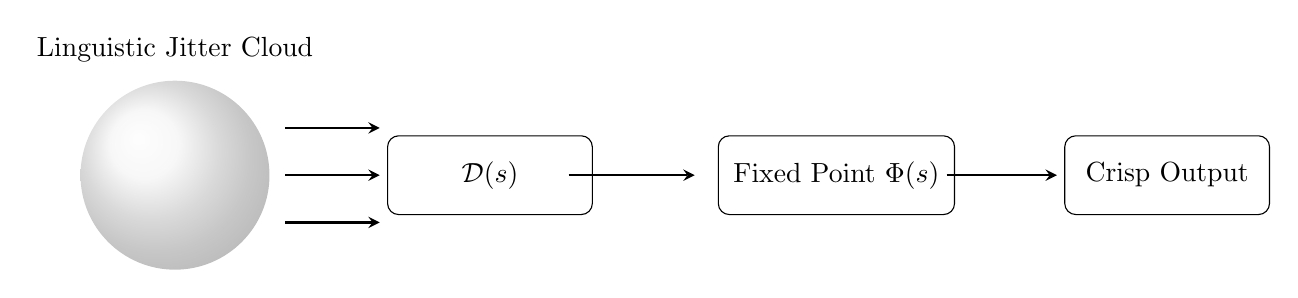
\begin{tikzpicture}[scale=1.0,>=stealth]
% Variance cloud
\shade[ball color=gray!20, opacity=0.4] (0,0) circle (1.2);
\node at (0,1.6) {Linguistic Jitter Cloud};

% Arrows from cloud to D(s)
\draw[->, thick] (1.4,0.6) -- (2.6,0.6);
\draw[->, thick] (1.4,0) -- (2.6,0);
\draw[->, thick] (1.4,-0.6) -- (2.6,-0.6);

% Node D(s)
\node[draw, rounded corners, minimum width=2.6cm, minimum height=1cm] at (4.0,0) {$\mathcal{D}(s)$};

% Arrow to Fixed point box
\draw[->, thick] (5.0,0) -- (6.6,0);
\node[draw, rounded corners, minimum width=3.0cm, minimum height=1cm] at (8.4,0) {Fixed Point $\Phi(s)$};

% Arrow to crisp output
\draw[->, thick] (9.8,0) -- (11.2,0);
\node[draw, rounded corners, minimum width=2.6cm, minimum height=1cm] at (12.6,0) {Crisp Output};

\end{tikzpicture}
\caption{DIFW reduces linguistic variance clouds into a stable fixed-point representation, which is then linearly projected to a crisp control parameter.}
\end{figure}

\section*{References}
\bibliographystyle{plainnat}
\begin{thebibliography}{9}

\bibitem[Jinek et~al.(2012)]{crisper}
Jinek, M., Chylinski, K., Fonfara, I., Hauer, M., Doudna, J. A., \& Charpentier, E. (2012).
A programmable dual-RNA-guided DNA endonuclease in adaptive bacterial immunity.
\textit{Science}, 337(6096), 816--821.

\bibitem[Wagner(2011)]{evo}
Wagner, A. (2011).
\textit{The Origins of Evolutionary Innovation}.
Oxford University Press.

\bibitem[Hofstadter \& Sander(2016)]{complex}
Hofstadter, D. R., \& Sander, E. (2016).
The deep structure of analogy in evolution.
\textit{Complex Systems Review}.

\end{thebibliography}

\end{document}

